\documentclass[journal,12pt,twocolumn]{IEEEtran}

\usepackage{setspace}
\usepackage{gensymb}
\singlespacing
\usepackage[cmex10]{amsmath}

\usepackage{amsthm}

\usepackage{mathrsfs}
\usepackage{txfonts}
\usepackage{stfloats}
\usepackage{float}
\usepackage{bm}
\usepackage{cite}
\usepackage{cases}
\usepackage{subfig}

\usepackage{longtable}
\usepackage{multirow}

\usepackage{enumitem}
\usepackage{mathtools}
\usepackage{steinmetz}
\usepackage{tikz}
\usepackage{circuitikz}
\usepackage{verbatim}
\usepackage{tfrupee}
\usepackage[breaklinks=true]{hyperref}
\usepackage{graphicx}
\usepackage{tkz-euclide}

\usetikzlibrary{calc,math}
\usepackage{listings}
    \usepackage{color}                                            %%
    \usepackage{array}                                            %%
    \usepackage{longtable}                                        %%
    \usepackage{calc}                                             %%
    \usepackage{multirow}                                         %%
    \usepackage{hhline}                                           %%
    \usepackage{ifthen}                                           %%
    \usepackage{lscape}     
\usepackage{multicol}
\usepackage{chngcntr}
\usepackage{float}
\restylefloat{table}

\DeclareMathOperator*{\Res}{Res}

\renewcommand\thesection{\arabic{section}}
\renewcommand\thesubsection{\thesection.\arabic{subsection}}
\renewcommand\thesubsubsection{\thesubsection.\arabic{subsubsection}}

\renewcommand\thesectiondis{\arabic{section}}
\renewcommand\thesubsectiondis{\thesectiondis.\arabic{subsection}}
\renewcommand\thesubsubsectiondis{\thesubsectiondis.\arabic{subsubsection}}


\hyphenation{op-tical net-works semi-conduc-tor}
\def\inputGnumericTable{}                                 %%

\lstset{
%language=C,
frame=single, 
breaklines=true,
columns=fullflexible
}
\begin{document}

\newcommand{\BEQA}{\begin{eqnarray}}
\newcommand{\EEQA}{\end{eqnarray}}
\newcommand{\define}{\stackrel{\triangle}{=}}
\bibliographystyle{IEEEtran}
\raggedbottom
\setlength{\parindent}{0pt}
\providecommand{\mbf}{\mathbf}
\providecommand{\pr}[1]{\ensuremath{\Pr\left(#1\right)}}
\providecommand{\qfunc}[1]{\ensuremath{Q\left(#1\right)}}
\providecommand{\sbrak}[1]{\ensuremath{{}\left[#1\right]}}
\providecommand{\lsbrak}[1]{\ensuremath{{}\left[#1\right.}}
\providecommand{\rsbrak}[1]{\ensuremath{{}\left.#1\right]}}
\providecommand{\brak}[1]{\ensuremath{\left(#1\right)}}
\providecommand{\lbrak}[1]{\ensuremath{\left(#1\right.}}
\providecommand{\rbrak}[1]{\ensuremath{\left.#1\right)}}
\providecommand{\cbrak}[1]{\ensuremath{\left\{#1\right\}}}
\providecommand{\lcbrak}[1]{\ensuremath{\left\{#1\right.}}
\providecommand{\rcbrak}[1]{\ensuremath{\left.#1\right\}}}
\theoremstyle{remark}
\newtheorem{rem}{Remark}
\newcommand{\sgn}{\mathop{\mathrm{sgn}}}
\providecommand{\abs}[1]{\vert#1\vert}
\providecommand{\res}[1]{\Res\displaylimits_{#1}} 
\providecommand{\norm}[1]{\lVert#1\rVert}
%\providecommand{\norm}[1]{\lVert#1\rVert}
\providecommand{\mtx}[1]{\mathbf{#1}}
\providecommand{\mean}[1]{E[ #1 ]}
\providecommand{\fourier}{\overset{\mathcal{F}}{ \rightleftharpoons}}
%\providecommand{\hilbert}{\overset{\mathcal{H}}{ \rightleftharpoons}}
\providecommand{\system}{\overset{\mathcal{H}}{ \longleftrightarrow}}
	%\newcommand{\solution}[2]{\textbf{Solution:}{#1}}
\newcommand{\solution}{\noindent \textbf{Solution: }}
\newcommand{\cosec}{\,\text{cosec}\,}
\providecommand{\dec}[2]{\ensuremath{\overset{#1}{\underset{#2}{\gtrless}}}}
\newcommand{\myvec}[1]{\ensuremath{\begin{pmatrix}#1\end{pmatrix}}}
\newcommand{\mydet}[1]{\ensuremath{\begin{vmatrix}#1\end{vmatrix}}}
\numberwithin{equation}{subsection}
\makeatletter
\@addtoreset{figure}{problem}
\makeatother
\let\StandardTheFigure\thefigure
\let\vec\mathbf
\renewcommand{\thefigure}{\theproblem}
\def\putbox#1#2#3{\makebox[0in][l]{\makebox[#1][l]{}\raisebox{\baselineskip}[0in][0in]{\raisebox{#2}[0in][0in]{#3}}}}
     \def\rightbox#1{\makebox[0in][r]{#1}}
     \def\centbox#1{\makebox[0in]{#1}}
     \def\topbox#1{\raisebox{-\baselineskip}[0in][0in]{#1}}
     \def\midbox#1{\raisebox{-0.5\baselineskip}[0in][0in]{#1}}
\vspace{3cm}
\title{AI1103--Assignment-2}
\author{Name: Aravinda Kumar Reddy Thippareddy\\Roll.No.:CS20BTECH11053}
\maketitle
\newpage
\bigskip
\renewcommand{\thefigure}{\theenumi}
\renewcommand{\thetable}{\theenumi}

\section*{Question}
Probability density function $p(x)$ of random variable x is as shown below. The value of a is
\begin{enumerate}[label=\Alph*)]
    \item $\frac{2}{c}$
    \item $\frac{1}{c}$
    \item $\frac{2}{(b+c)}$
    \item $\frac{1}{(b+c)}$
\end{enumerate}
\begin{figure}[H]
\centering
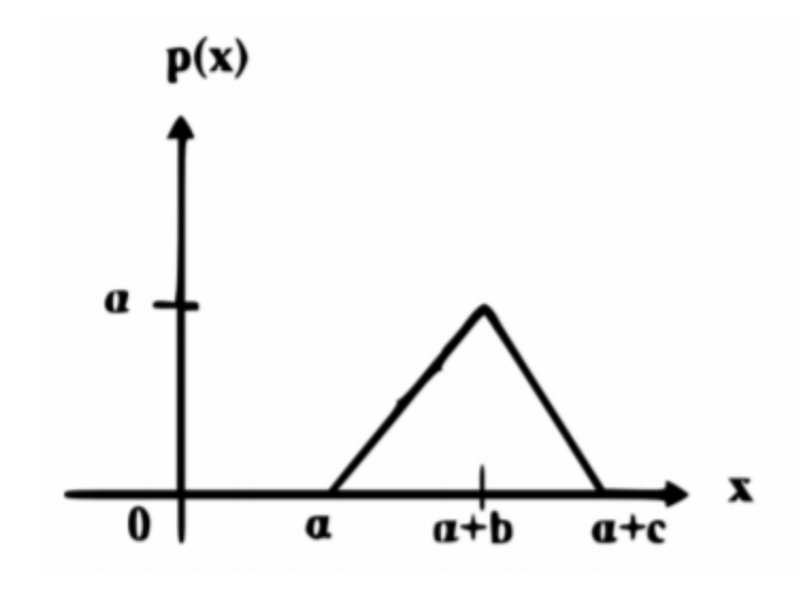
\includegraphics[width=\columnwidth]{Screenshot_20210403-145019.png}
\caption{PDF}
\label{fig:convolution}
\end{figure}
\section*{Solution}
Let $Y_1$ and $Y_2$ be two independent and identically distributed (IID) uniform random variables.\\
Let X be a random variable such that
\begin{align}
    X = Y_1 + Y_2
\end{align}
Let
\begin{align}
    p_{Y_1}\brak{y} &= \Pr\brak{Y_1=y} \\
    p_{Y_2}\brak{y} &= \Pr\brak{Y_2=y} \\
    p_X\brak{x} &= \Pr\brak{X=x}
\end{align}
be the probability densities of random variables $Y_1, Y_2$ and $X$. \\
$Y_1$ and $Y_2$ lie in the range \brak{\frac{-c}{4},\frac{c}{4}}, therefore, the PDF for $Y_1$ and $Y_2$,
\begin{align}
p_{Y_1}\brak{y} = p_{Y_2}\brak{y} = 
\begin{cases}
\frac{2}{c} &  \frac{-c}{4} \le y \le \frac{c}{4}\\
0 & \text{otherwise}
\end{cases}
\end{align}
The density of X is obtained by convolution of $Y_1$ and $Y_2$
\begin{align}
p_X\brak{x} = p_{Y_1}(x)*p_{Y_2}(x)
\end{align}
where $*$ denotes the convolution operation. Since convolution operation is time invariant, 
\begin{multline}
    p_X\brak{x-t} = p_{Y_1}(x-t)*p_{Y_2}(x) \\ = p_{Y_1}(x)*p_{Y_2}(x-t)
\end{multline}
On time shifting $Y_1$ by shifting factor $t=a+\frac{c}{2}$, 
\begin{align}
    p_X\brak{x-\brak{a+\frac{c}{2}}} =  p_{Y_1}\brak{x-\brak{a+\frac{c}{2}}}*p_{Y_2}\brak{x}
\end{align}
Thus, the PDF of time shifted X obtained by convolution is,
\begin{align}
p_x = 
\begin{cases}
\frac{4}{c^2}\brak{x-a} & a \le x \le a+\frac{c}{2}\\
\frac{4}{c^2}\brak{a+c-x} & a+\frac{c}{2} \le x \le a+c \\
0 & \text{otherwise}
\end{cases}
\end{align}
On comparing the parameters of PDF of time shifted X with that in the question, we have
\begin{align}
    b=\frac{c}{2}\\
    a=\frac{2}{c}
\end{align}
\rightline{Answer : Option A}
\begin{figure}[H]
\centering
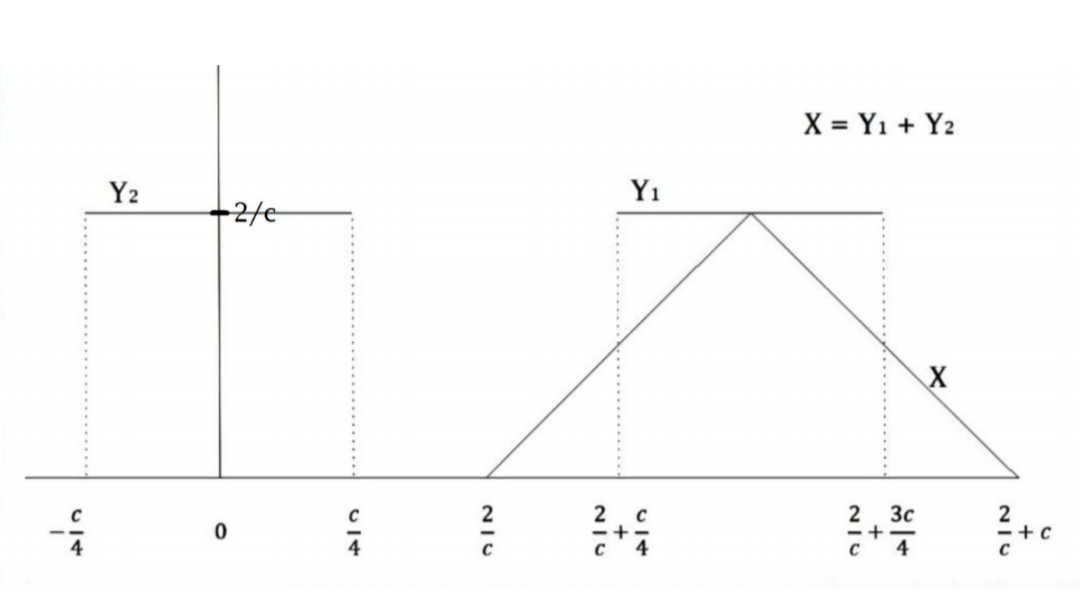
\includegraphics[width=\columnwidth]{Screenshot_20210403-145122.png}
\caption{PDF of time shifted X}
\label{fig:con6}
\end{figure}
The following are some observations: 
\begin{enumerate}
    \item The sum of two equally distributed random variables will lead to a triangular probability density
    \item The two uniformly distributed random variables lie in the range $\brak{\frac{-c}{4},\frac{c}{4}}$ and $\brak{\frac{2}{c}+\frac{c}{4} , \frac{2}{c}+\frac{3c}{4}}$. \\
    \because $X = Y_1 + Y_2$ the range of X is thus $\brak{\frac{2}{c},\frac{2}{c}+c}$
    \item On time shifting $Y_1$ to the right by a factor $a+\frac{c}{2}$, the convoluted PDF of X also shifts by the same factor without any change in it's width.
\end{enumerate}
Fig \ref{fig:sim3} and Fig \ref{fig:sim4} are the plots of PDF and CDF obtained by taking c=2
\begin{figure}[H]
\centering
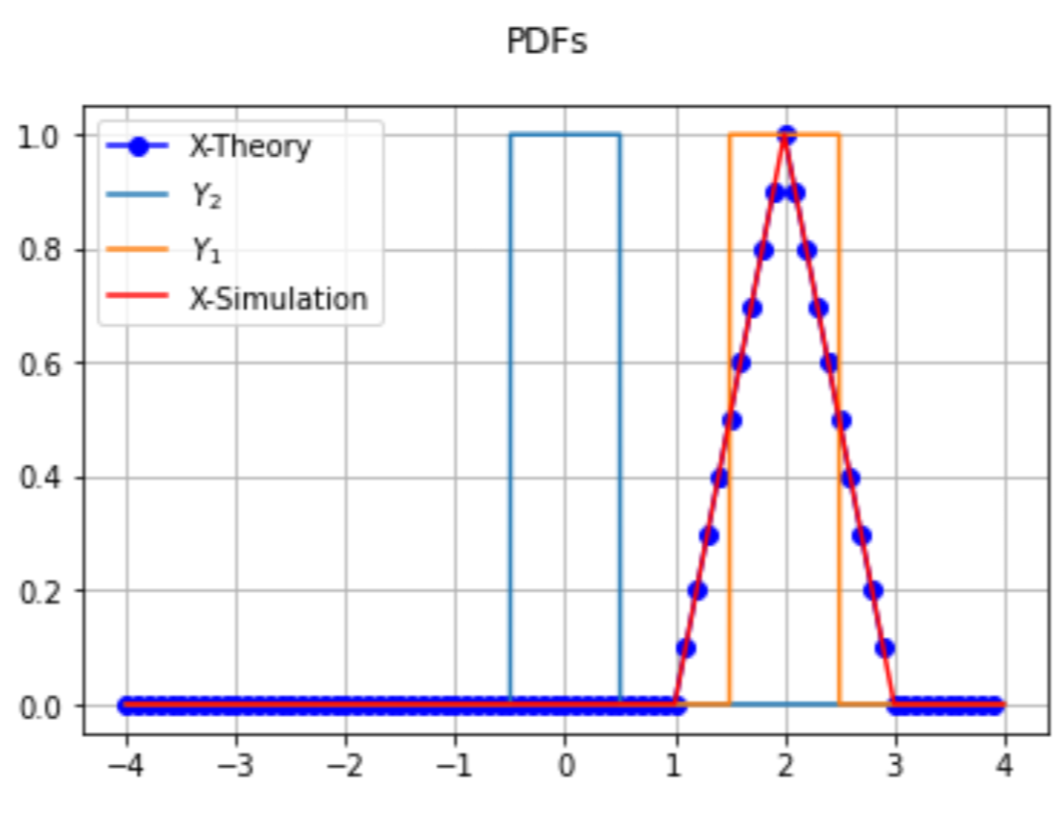
\includegraphics[width=\columnwidth]{Screenshot_20210403-210159.png}
\caption{PDF of $Y_1, Y_2$ and X}
\label{fig:sim3}
\end{figure}
\begin{figure}[H]
\centering
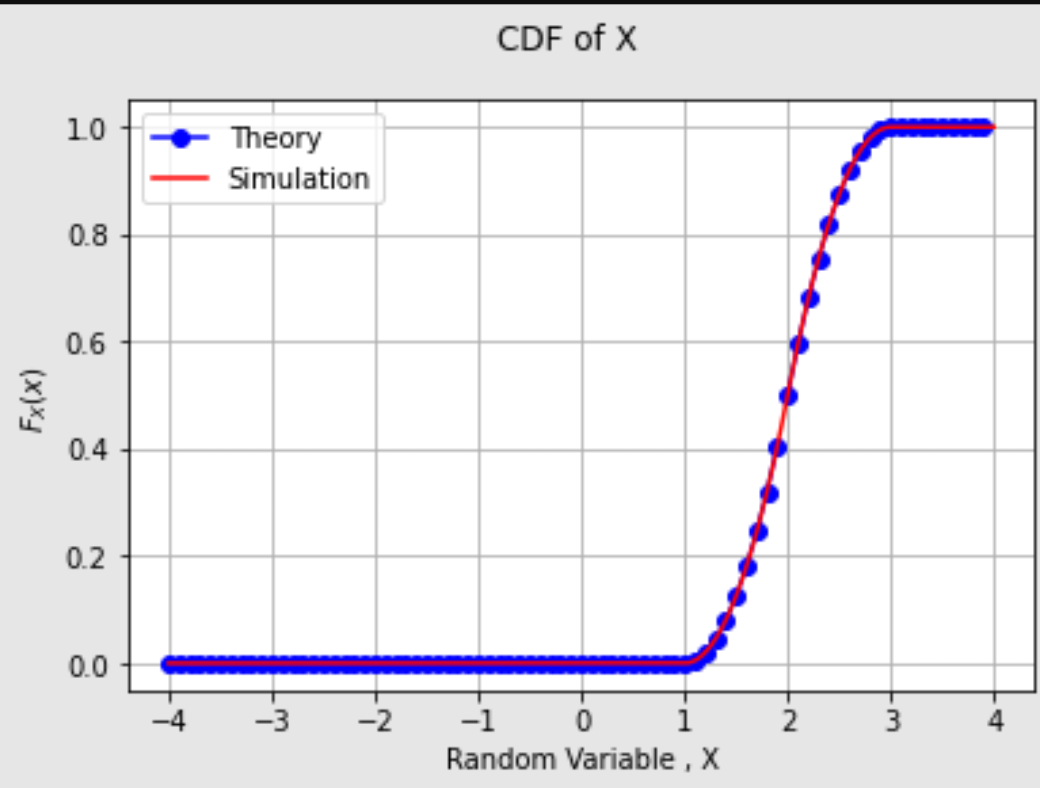
\includegraphics[width=\columnwidth]{Screenshot_20210403-210223.png}
\caption{CDF of X}
\label{fig:sim4}
\end{figure}
\end{document}